% ============================================================
\appendix
\section*{Appendix A. Category-Theoretic Background}
\addcontentsline{toc}{section}{Appendix A. Category-Theoretic Background}
% ============================================================

This appendix summarizes the categorical notions used in the paper.
It is intended for readers with a background in data modeling,
databases, or formal methods who may not use category theory daily.
The goal is conceptual clarity rather than mathematical depth.

% ------------------------------------------------------------
\subsection*{A.1 Categories}
% ------------------------------------------------------------

A \emph{category} consists of:
\begin{itemize}
    \item a collection of \textbf{objects};
    \item a collection of \textbf{morphisms} (arrows) between objects;
    \item an associative composition operation
          and an identity arrow for each object.
\end{itemize}

Intuition:
\begin{itemize}
    \item Objects represent states or structured data (e.g., CEP records).
    \item Morphisms represent valid transformations (e.g., amendments).
    \item Composition corresponds to applying transformations sequentially.
\end{itemize}

\medskip
Example:
A sequence of record updates in CEP corresponds to a chain of morphisms
\[ R_0 \to R_1 \to R_2 \to \cdots. \]

% ------------------------------------------------------------
\subsection*{A.2 Functors}
% ------------------------------------------------------------

A \emph{functor} $F : \mathbf{C} \to \mathbf{D}$ maps:
\begin{itemize}
    \item each object of $\mathbf{C}$ to an object of $\mathbf{D}$,
    \item each morphism in $\mathbf{C}$ to a morphism in $\mathbf{D}$,
\end{itemize}
such that identities and composition are preserved.

Intuition:
\begin{itemize}
    \item A functor is a structure-preserving translation.
    \item CEP uses functors to model processes such as
          envelope construction or canonicalization.
\end{itemize}

% ------------------------------------------------------------
\subsection*{A.3 Natural Transformations}
% ------------------------------------------------------------

Given functors $F, G : \mathbf{C} \to \mathbf{D}$,
a \emph{natural transformation} $\eta : F \Rightarrow G$ assigns
to each object $X$ in $\mathbf{C}$ a morphism
\[
\eta_X : F(X) \to G(X)
\]
such that each square
\[
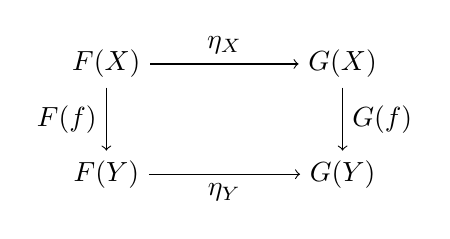
\begin{tikzpicture}[baseline=(current bounding box.center)]
\node (FX) at (0,0) {$F(X)$};
\node (GX) at (3,0) {$G(X)$};
\node (FY) at (0,-1.4) {$F(Y)$};
\node (GY) at (3,-1.4) {$G(Y)$};
\draw[->] (FX) -- node[above] {$\eta_X$} (GX);
\draw[->] (FY) -- node[below] {$\eta_Y$} (GY);
\draw[->] (FX) -- node[left] {$F(f)$} (FY);
\draw[->] (GX) -- node[right] {$G(f)$} (GY);
\end{tikzpicture}
\]
commutes for all morphisms $f : X \to Y$.

Intuition:
\begin{itemize}
    \item Naturality means: \emph{"attest first then transform" =
          "transform first then attest"}. 
    \item This is exactly the coherence needed for CEP attestation chains.
\end{itemize}

% ------------------------------------------------------------
\subsection*{A.4 Monoidal Categories}
% ------------------------------------------------------------

A \emph{monoidal category} is a category equipped with:
\begin{itemize}
    \item a tensor product $\otimes$ combining objects,
    \item a unit object $I$,
    \item coherence laws ensuring associativity and proper unit behavior.
\end{itemize}

In CEP, the relevant monoidal structure is \textbf{string concatenation}:
\begin{itemize}
    \item canonical components (name, address, date) combine via $\otimes$,
    \item the canonicalization functor preserves this structure strictly.
\end{itemize}

This allows the SNFEI to be treated as a universal construction.

% ------------------------------------------------------------
\subsection*{A.5 Oplax Functors}
% ------------------------------------------------------------

Given monoidal categories $(\mathbf{C}, \otimes)$ and $(\mathbf{D}, \otimes)$,
an \emph{oplax monoidal functor} $F : \mathbf{C} \to \mathbf{D}$ comes with
coherence maps
\[
F(X) \otimes F(Y) \to F(X \otimes Y)
\]
that need not be invertible.

Intuition:
\begin{itemize}
    \item Oplax functors allow \textbf{structure weakening}.
    \item This directly models jurisdictional adapters:
          some structure from the local schema may be incomplete or
          only partially mappable to the global vocabulary.
\end{itemize}

% ------------------------------------------------------------
\subsection*{A.6 Indexed Families and Fibrations}
% ------------------------------------------------------------

A \emph{fibration} $\pi : \mathbf{E} \to \mathbf{B}$ consists of:
\begin{itemize}
    \item a base category $\mathbf{B}$,
    \item a total category $\mathbf{E}$,
    \item a projection functor $\pi$,
    \item satisfying certain lifting properties.
\end{itemize}

The fiber over $B \in \mathbf{B}$ is the category
\[
\mathbf{E}_B = \{ E \in \mathbf{E} \mid \pi(E) = B \}.
\]

Intuition for CEP:
\begin{itemize}
    \item $\mathbf{B} = \mathbf{CEP}$ (identity-bearing records),
    \item $\mathbf{E} = \mathbf{CT}$ (records plus context tags),
    \item the fiber over $R$ is the set of all allowed context tags for $R$,
    \item fibers reindex naturally when $R$ evolves.
\end{itemize}

This formalizes the idea that context tags do not affect identity.

% ------------------------------------------------------------
\subsection*{A.7 Universal Properties (Informal)}
% ------------------------------------------------------------

A universal property specifies an object uniquely up to isomorphism
by the role it plays in relation to others.

In CEP:
\begin{itemize}
    \item the canonical string is universal for its admissible class
          of normalized components,
    \item the SNFEI is obtained by applying a hashing endofunctor,
    \item identity preservation follows from the uniqueness of the
          universal construction.
\end{itemize}

\bigskip
This concludes the appendix. Readers seeking more detail may consult
Mac~Lane~\cite{maclane1971categories},
Awodey~\cite{awodey2010category},
and Spivak~\cite{spivak2014category}.
